\documentclass[pdf]{prosper}
% for printing
%\documentclass[ps2pdf]{prosper}
% for using Acrobat Distiller
%\documentclass[pdf,distiller]{prosper}

% Introduction to the `HA-Prosper' package.
% Created by: Hendri Adriaens
%             http://center.uvt.nl/phd_stud/adriaens
%             Center for Economic Research
%             Tilburg University, the Netherlands

%================================================
% Please also read the manual of HA-prosper and
% of the specific style you are using since some
% features of this example might not be supported
% by the style you use.
%================================================

\usepackage[toc,hlsections,highlight,Cornell]{HA-prosper}

\HAPsetup{%
trans=Wipe,
tsnav=FullScreen,
nsnav=ShowBookmarks,
lf={\href{mailto:lars.vilhuber@cornell.edu}{Lars Vilhuber}, John Abowd and
  Bryce Stephens},
rf={\today},
iacolor=gray,
stype=1
}


% etc. 
\newcommand{\mytitle}{The LEHD Infrastructure Files}
\newcommand{\mysubtitle}{and the Creation of the Quarterly Workforce Indicators} 
\newcommand{\myshorttitle}{LEHD/ QWI Overview }
\newcommand{\myauthors}{John M. Abowd{\footnotesize
    $^{\spadesuit,\clubsuit}$},
 Bryce  E. Stephens{\footnotesize$^\clubsuit$} and 
 Lars Vilhuber{\footnotesize$^\spadesuit$}}%,\\with Fredrik Andersson, Kevin L. McKinney, Marc Roemer, and Simon Woodcock}
%\newcommand{\myversion}{January 22 2002}
%\papernumber{2002-02}
 \newcommand{\myversion}{\today}  %alternate version

\title{\mytitle}
\subtitle{\mysubtitle}
\author{\myauthors\\
\institution{$\spadesuit$ Cornell University}\\
\institution{$\clubsuit$ U.S. Census Bureau, LEHD Program}}


\begin{document}
\overlays{6}{%
  \begin{slide}{Data flow}
  \onSlide*{1}{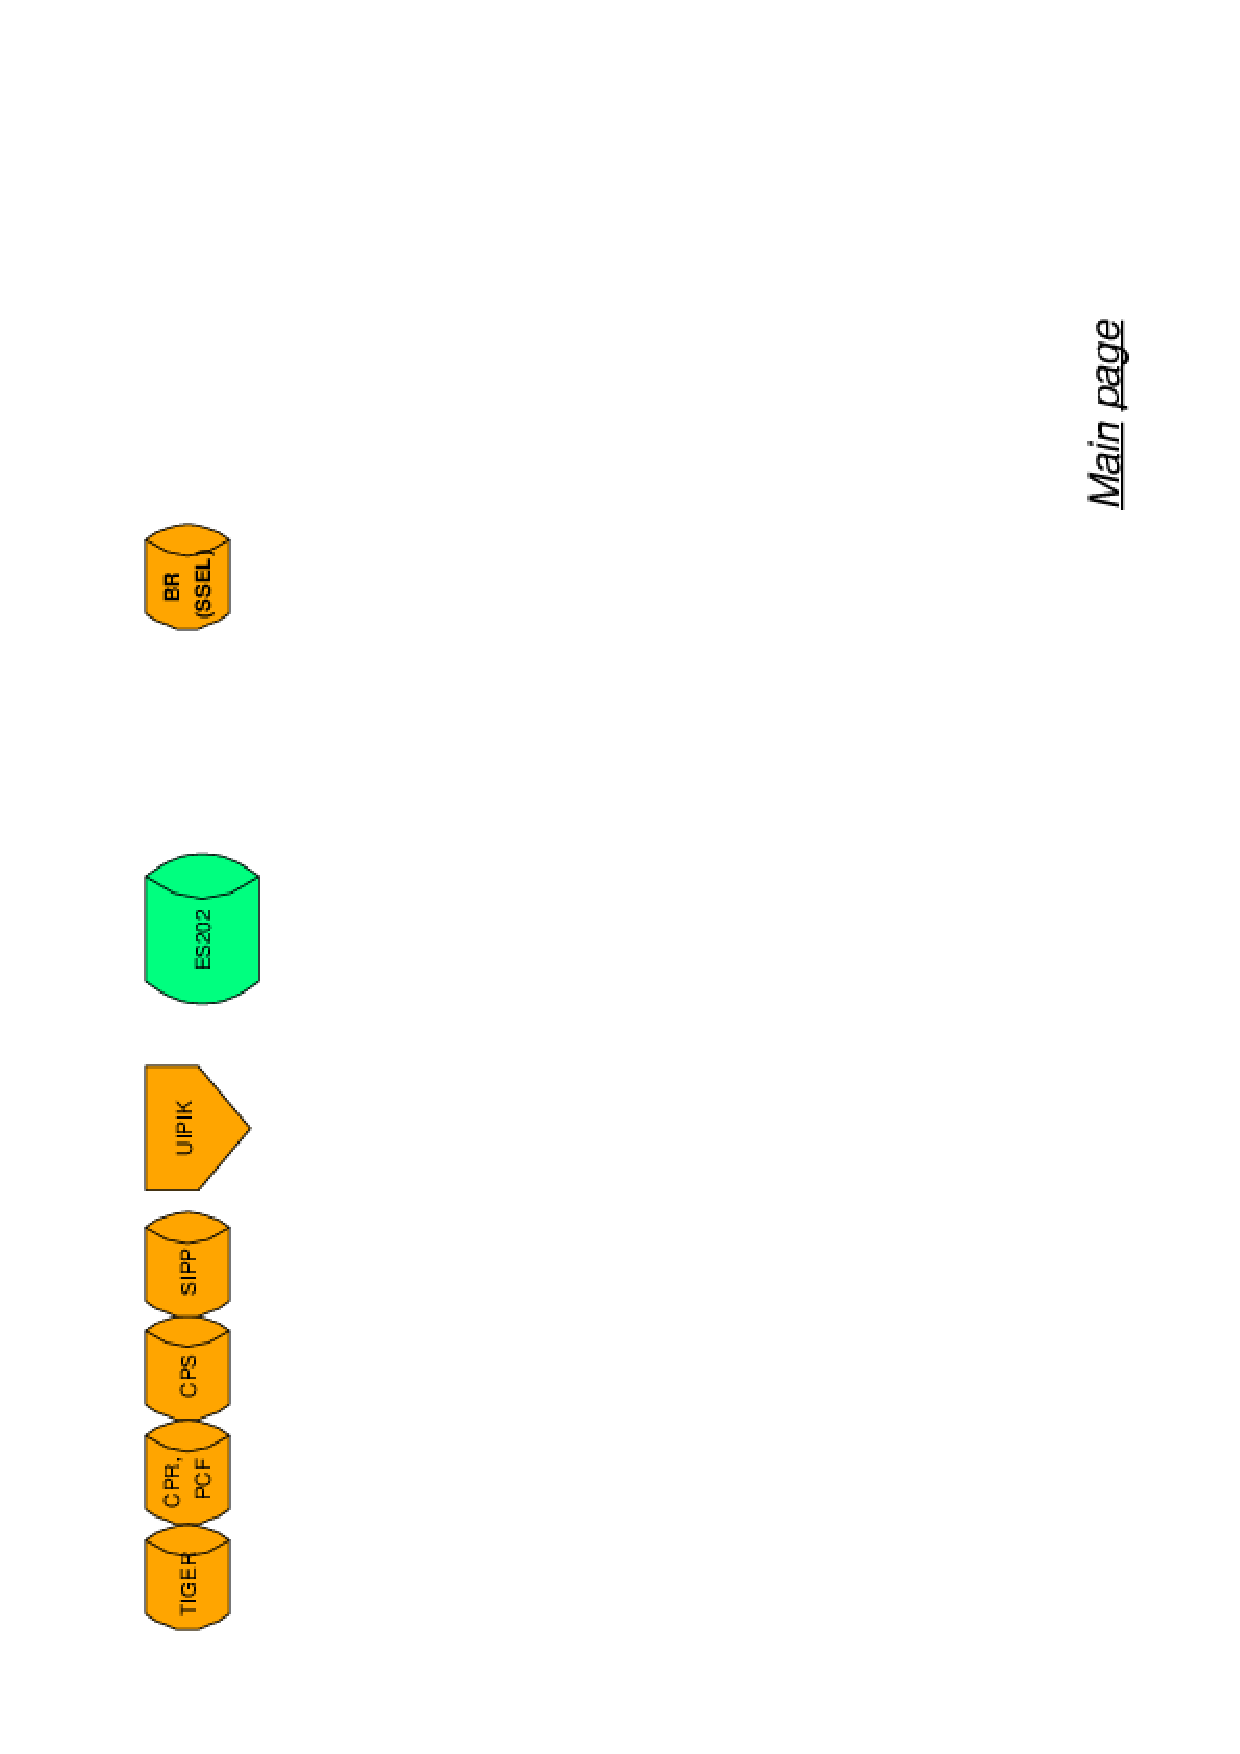
\includegraphics[scale=0.31,angle=270]{overview-data-flow/overview-data-flow-extract-stage0}}
  \onSlide*{2}{\includegraphics[scale=0.31,angle=270]{overview-data-flow/overview-data-flow-extract-stage1}}
  \onSlide*{3}{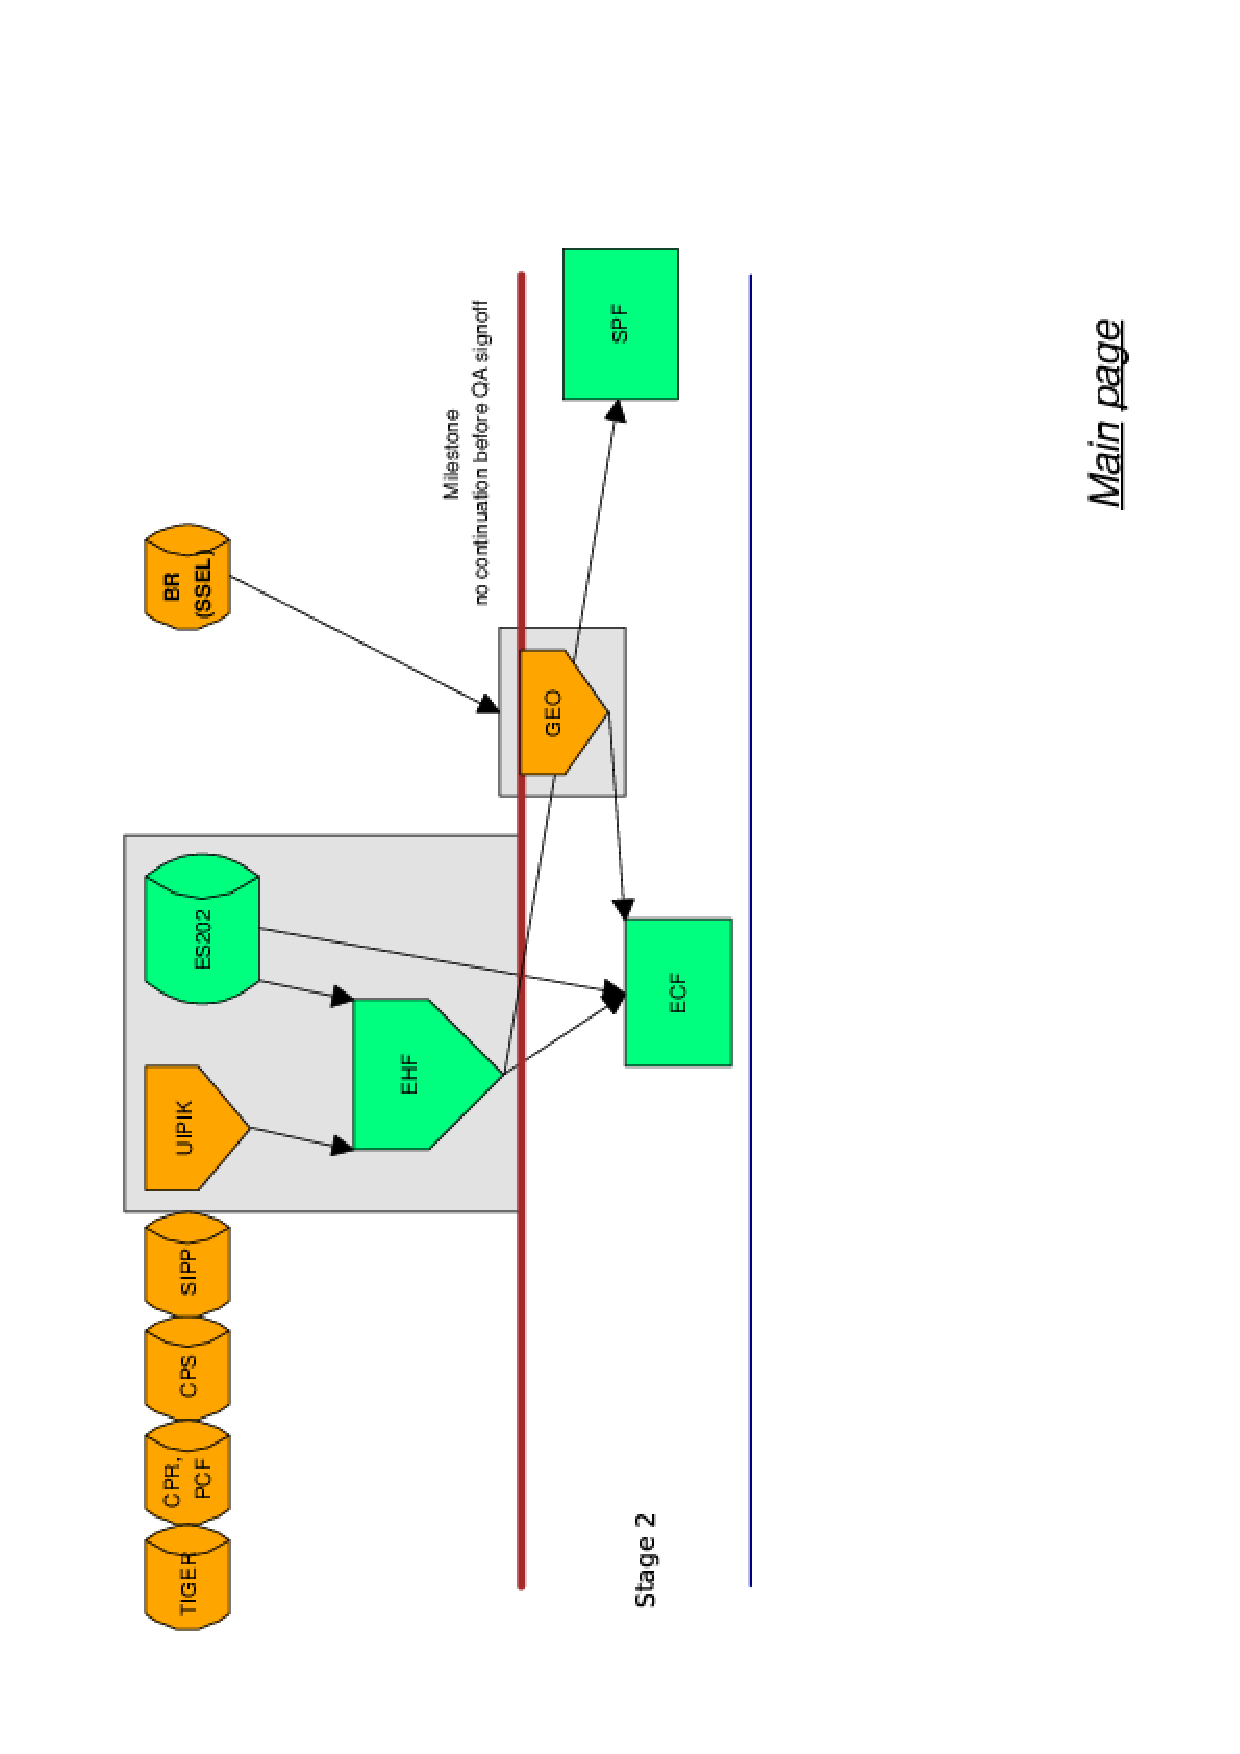
\includegraphics[scale=0.31,angle=270]{overview-data-flow/overview-data-flow-extract-stage2}}
  \onSlide*{4}{\includegraphics[scale=0.31,angle=270]{overview-data-flow/overview-data-flow-extract-stage3}}
  \onSlide*{5}{\includegraphics[scale=0.31,angle=270]{overview-data-flow/overview-data-flow-extract-qwi}}
  \onSlide*{6}{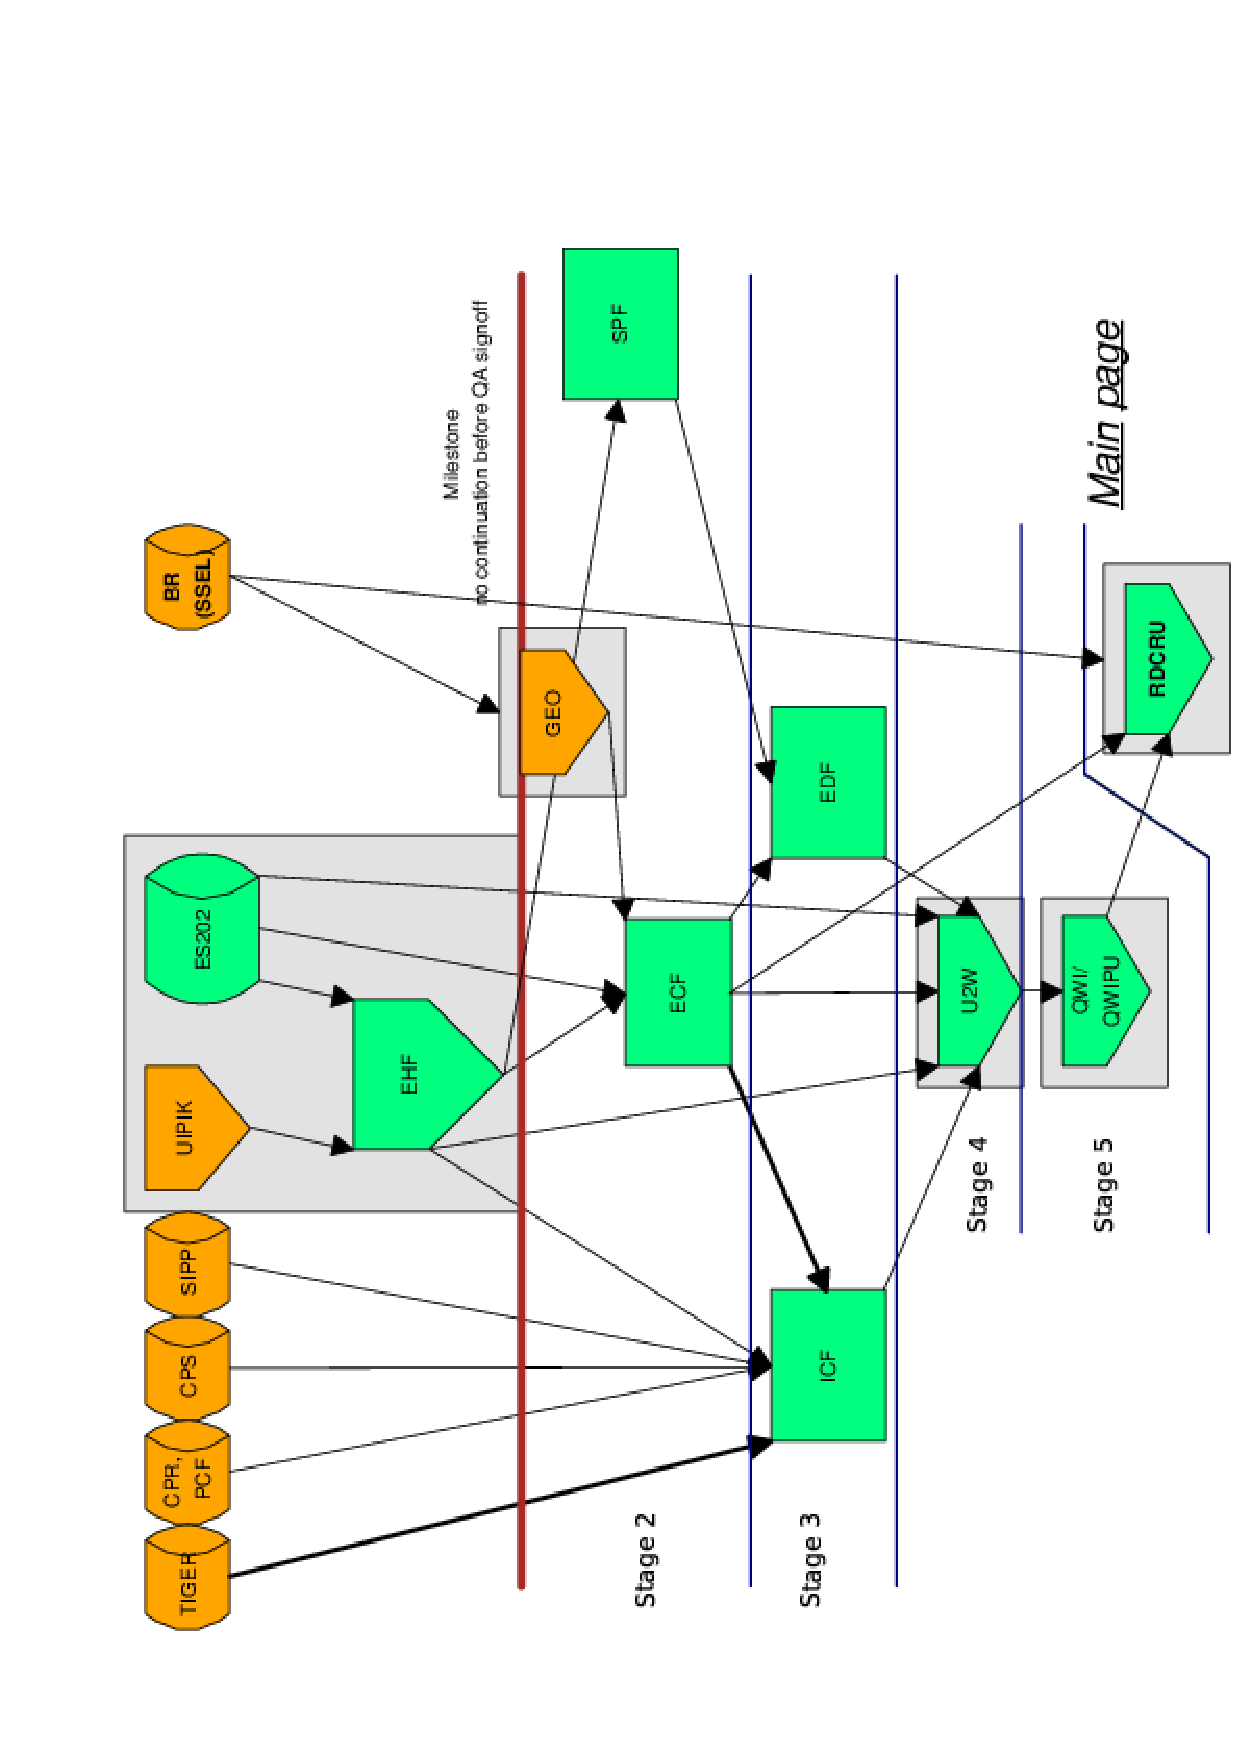
\includegraphics[scale=0.31,angle=270]{overview-data-flow/overview-data-flow-final}}
  \end{slide}
}

\overlays{1}{%
  \begin{slide}{QWI Detail}
  \onSlide*{1}{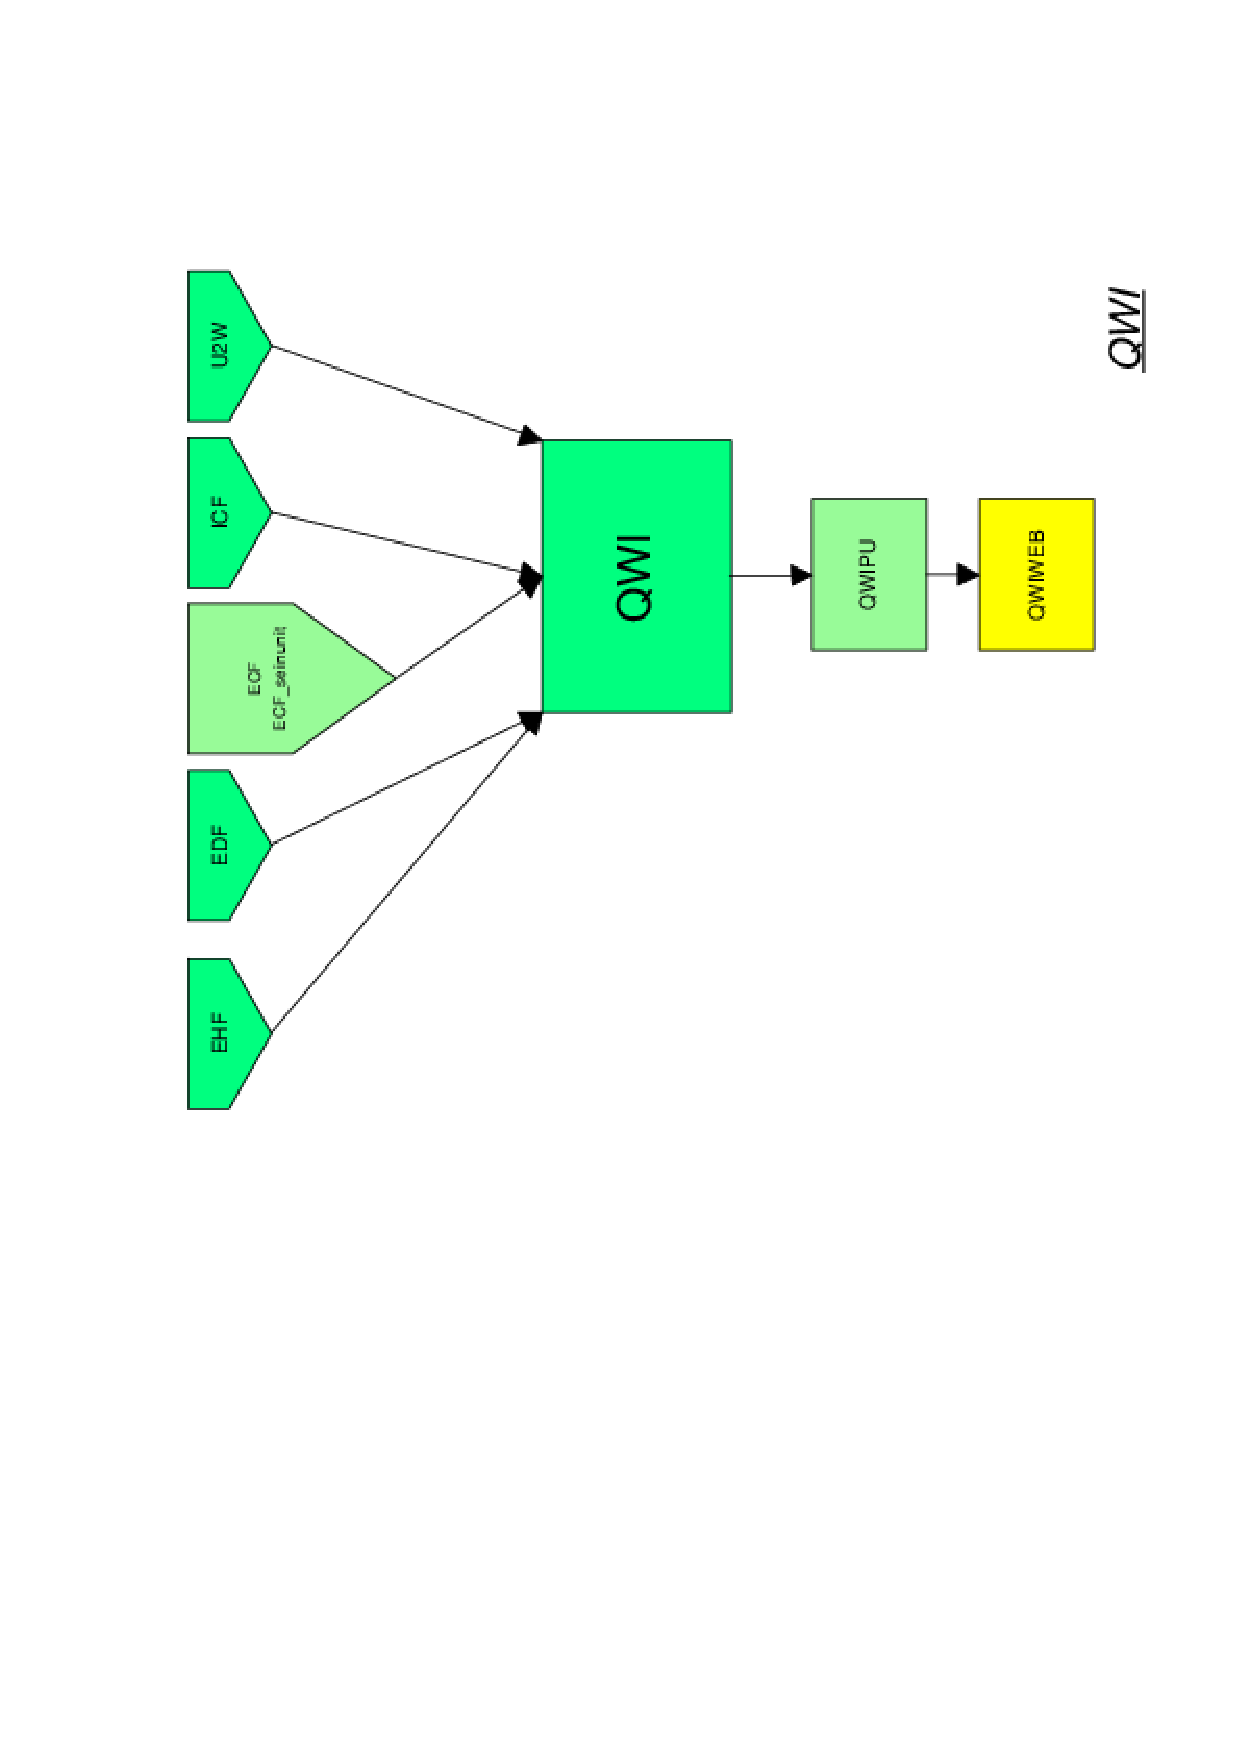
\includegraphics[scale=0.31,angle=270]{overview-data-flow/overview-data-flow-qwi}}
  \end{slide}
}
\overlays{1}{%
  \begin{slide}{Public Use Files}
  \onSlide*{1}{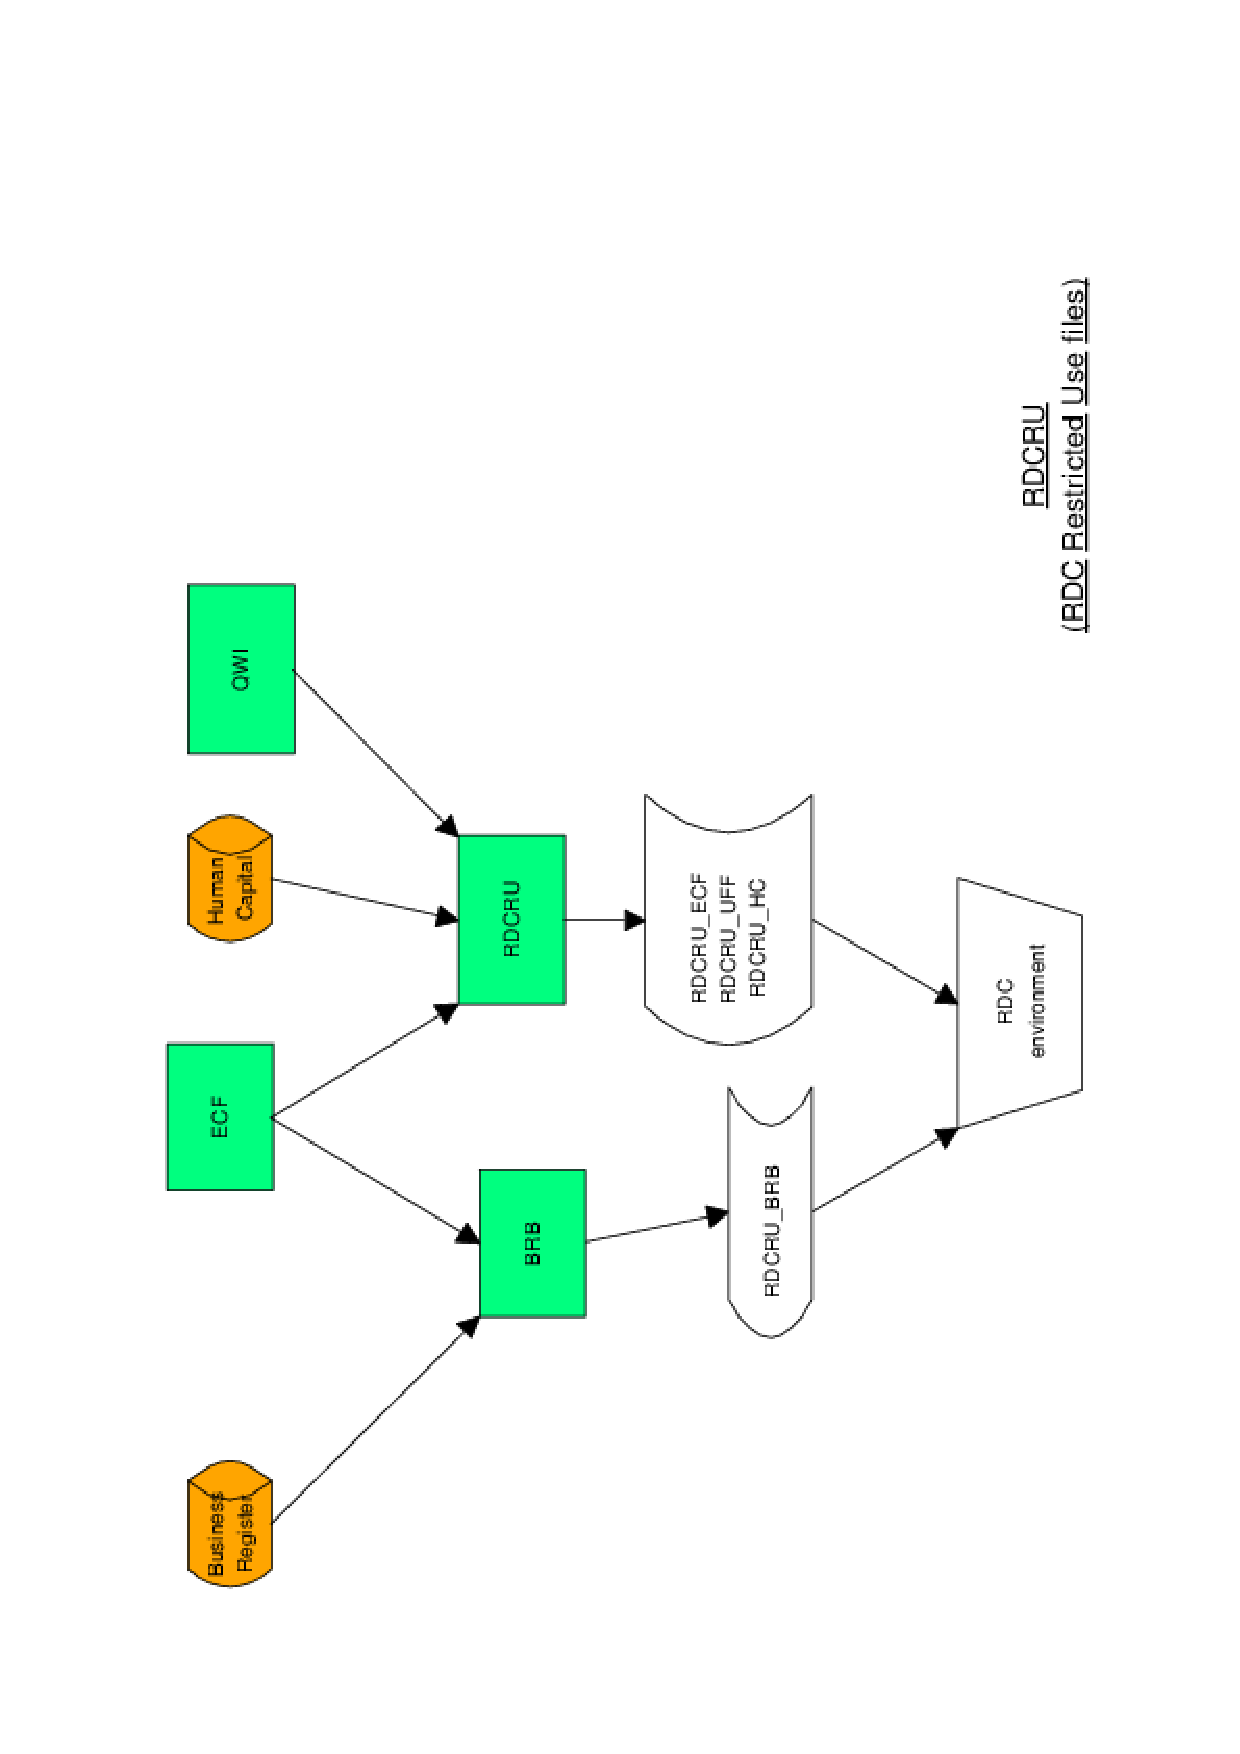
\includegraphics[scale=0.31,angle=270]{overview-data-flow/overview-data-flow-rdcru}}
  \end{slide}
}

\end{document}
